\textbf{Trenger jeg denne biten? Evt hvor?}
In this one year long project, we have collected results of a great number of materials with various structures and compositions. The initial experimentation was based on high-entropy silicides of the $Fe_2Si$ unit cell, created from the special quasi-random structure approach as described above. Despite the non-semiconducting character of this compound, we worked under the idea that the extraordinary properties that have been observed in high-entropy alloys through effects such as the cocktail effect, we could discover specific combinations of elements that would yield a semiconductor. In addition, the ratio between silicon atoms to metals allowed us to create nearly eqvimolar high-entropy alloys. 

Following this attempt, we transistioned into studying high-entropy silicides based on well known semiconducting 3d silicides such as $\beta-$\ch{FeSi2}, \ch{CrSi2} and \ch{MnSi_{1.75}}. The main outcome of this project is that for all 4 different starting silicides, we could only produce high-entropy silicides from one unit cell, furthermore in this cell only one specific compositions of elements was semiconducting. This was \ch{Cr_{0.25}Fe{0.25}Mn_{0.25}Ni_{0.25})Si2}, here-in CFMN, in the $\beta-$ \ch{FeSi2} crystal structure.  

This section will be structured in the following manner, firstly we will investigate the CFMN (fesi2) compound and various permutations of the composition. Thereafter we will look at other possible compositions of fesi2 based high-entropy silicides, and lastly test the CFMN composition in other crystal symmetries. In final we will present an overview of the complete study and the various compounds that have been investigated in order to propose promising directions and guideline future research directions in this field. In this way, we aim to understand the uniqe properties of CFMN (fesi2) and why this particular compound is semiconducting compared to the other testes structures in this project. Properties we will cover is the overall stability by total energy and corresponding enthalpy of formation, the magnetic properties and which elements contribute to the magnetism. But in majority, we will look at the band gap and related properties, as this is the main motivation and distinction of the study.    

\chapter{The good (CFMN fesi2)}
\label{sec:good}

$\beta-FeSi_2$ in the orthorombic cmce crystal lattice is a well known semiconductor with an experimentally measured band gap of around 0.8 ev \textbf{cite}, the nature of the band gap is under debate, all though most ab inito studies point to an indirect gap, experimental work indicate a direct gap. From our own DFT calculations, we find an indirect band gap close to 0.65 eV with PBE. This is in good agreement with other meassurements from ab intitio studies \textbf{cite materials projects, other studies.} 

The density of states and charge density of bulk $\beta-$\ch{FeSi2} from PBE calculations can be seen in figure .., ..  From the figures we observe a clear band gap and semiconducting character. Moreover, we note from the density of states that the gap is identical in both spin channels, indicating that this material is diamagnetic. We find this to be true from the written magnetization in VASP, this also is in agreement with relevant literature \textbf{cite}. \textbf{Find reference for stability and $\Delta H^0$.} Finally, the enthalpy of formation of this compound is -18.6583 eV.

\section{CFMN Eqvimolar distribution}

\subsection{Introduction}

The CFMN alloys of the fesi2 unit cell alloys can be seen in figure ... The supercells consist of 48 atoms, 16 of which is evenly distributed between Cr, Fe, Mn, and Ni, the remaining 32 sites occupied by silicon atoms. Bellow in table .. we list the total energy per atom (Toten), final magnetic moment per atom (Mag), and the band gap of the five distinct SQSs corresponding to the CFMN (fesi2) compound. In addition we include the mean and standard deviation of the values, plus the enthalpy of formation. For simplicity, we denote the SQSs as A, B, C, D and E.

\begin{table}[H]
\centering
\begin{tabular}{@{}cccc@{}}
\toprule
Structure  & Toten (eV) & Mag (?) & Band gap (eV) \\ \midrule
\textbf{A} & −6,6080                & 0.0833                    & 0.0280        \\
\textbf{B} & −6,6138                & 0.0833                    & 0.0523        \\
\textbf{C} & −6,6063                & 0.0834                    & 0.0344        \\
\textbf{D} & −6,6155                & 0.0833                    & 0             \\
\textbf{E} & −6,6089                & 0.0833                    & 0.0495        \\ \midrule
\textbf{Mean} & -6.6105 & 4.0000 & 0.0328    \\
\textbf{Std} & 0.0039 &  0.0000 &  0.0210 \\
\textbf{$\Delta H_{mean}^0$} & -11.5000 eV & - & - \\ \bottomrule
\end{tabular}
\caption{Total energy per atom, final magnetic moment, band gap (GGA) and formation enthalpy of $Cr_4Fe_4Mn_4Ni_4Si_{32}$ SQSs based on $FeSi_2$}
\label{table:fesi2_summary}
\end{table}  

\textbf{Write a section on magnetism in method}
From a first glance, we observe very similar properties between the SQSs regarding both the total energy and final magnetic moment. Comparing to bulk \ch{FeSi_2}, this compound is both less stable, from the enthalpy of formation, and magnetic. For the magnetic character of the compound, we performed self-consistent total energy calculations with three diffrent magnetic configurations, non-magnetic (ispin=1), colinear magnetism with the initial magnetic moment equal to 1 times the number of ions, and lastly two times N ions. Of the three starting positions, we found the two latter to yield near identical total energies, with the middle seting winning out in some SQSs. The consistent magnetic moment between the 5 supercells is excpected seeing as all 5 structures consist of equivalent elements. The magnetic moment observed is solely attributed from 3d electrons and in particular those of chromium and manganese atoms. 
 
\subsection{The band gap} 
 
The most interesting property of these SQSs is in fact the band gap. We note a mean band gap of about 0.03 eV, much lower than 0.65 eV of bulk $FeSi_2$. But a band gap in this smaller range makes for  excellent application in for instance thermoelectrics. The gap is seen in 4 out of 5 SQSs, but surprisingly not in the most stable arrangement (D), the largest gap observed is about 0.05 eV from structure B, which is slighlty bellow D in terms of total energy, but still a way above the mean energy. Similar to the bulk material, also these band gaps are indirect, the transitions are listed bellow in table .. .     

\begin{table}[H]
\centering
\begin{tabular}{@{}ccc@{}}
\toprule
Structure  & Gap (D/I) & Transition                              \\ \midrule
\textbf{A} & I         & (0.500,0.333,0.500) $\rightarrow$ (0.500,0.000,0.000)  \\
\textbf{B} & I         & (0.250,0.000,0.250) $\rightarrow$ (0.000,0.000,0.000)  \\
\textbf{C} & -         & (0.500,0.000,0.500) $\rightarrow$ (-0.250,0.333,0.500) \\
\textbf{D} & I         & -                                        \\
\textbf{E} & I         & (0.000,0.000,0.000) $\rightarrow$ (0.250,0.000,0.250)  \\ \bottomrule
\end{tabular}
\caption{Band gap transition of CFMN (fesi2) SQSs with PBE functional}
\end{table}

A very useful method to extract information regarding the band gap of a material is to plot and study the band structure, however this is not as insightful when considering large supercells consisting of several elements and a  large number of energy bands. The solution to this is normally to do a band unfolding, but given the complex structure and implementation of these SQS is VASP we where not able to do either. Instead we can study the band gap by firstly observing the density of states, in figure .. we plot both the total density of states (TDOS) and the local density of states (LDOS) of SQS D.

\begin{figure}[H]
	\centering
	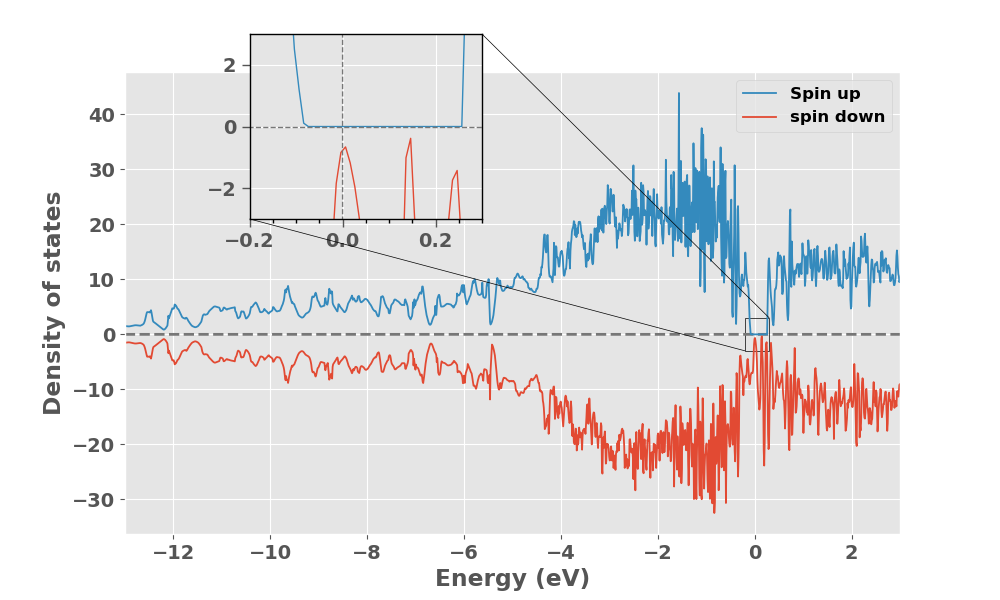
\includegraphics[width=\textwidth]{results/fesi2/D_TDOS.png}
	\caption{Density of states SQS D CFMN (fesi2) from PBE calculation}
\end{figure}

From TDOS we learn that D is in fact a half-metal with a sizable band gap in the spin $\uparrow$ channel, and a metal in spin $\downarrow$. From the local density of states we observe that states corresponding to energies much lower than $E_F$ is dominated by the s electrons of silicon atoms. At slightly higher energies, we see strong hybridization of Si p electrons and TM 3d electrons. In both spin channels Ni lie at the lowest energies of the 3d elements, followed by iron and then manganese and chromium very close to the fermi energi. Above the fermi enery there is more of an equal contribution from all elements, however slightly above Ef particularly iron and chromuim show a distinction in spin up and down respectfully.  At higher energies, the LDOS is attributed to Si and Cr in both spin states, while elements such as Ni, Fe and Mn have  a lesser role on the total DOS. One key distinction of str D is a heavy amount of Manganese at energies right above Ef in spin down, this is not the case in the other SQSs (Appendix A). An additional distinction is that we observe higher overall peaks in the local density of states in the semicondcing SQSs B and e, compared to D. 

\begin{figure}[H]
	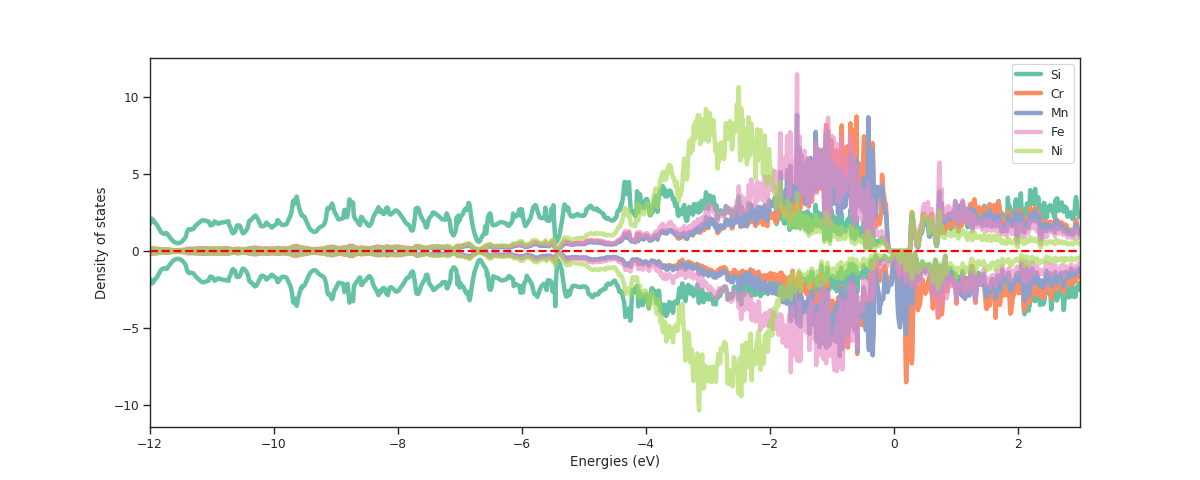
\includegraphics[width=\textwidth]{results/fesi2/D_LDOS.png}
	\caption{Local density of states SQS D CFMN (fesi2) from PBE calculation}
\end{figure}

\begin{figure}[H]
	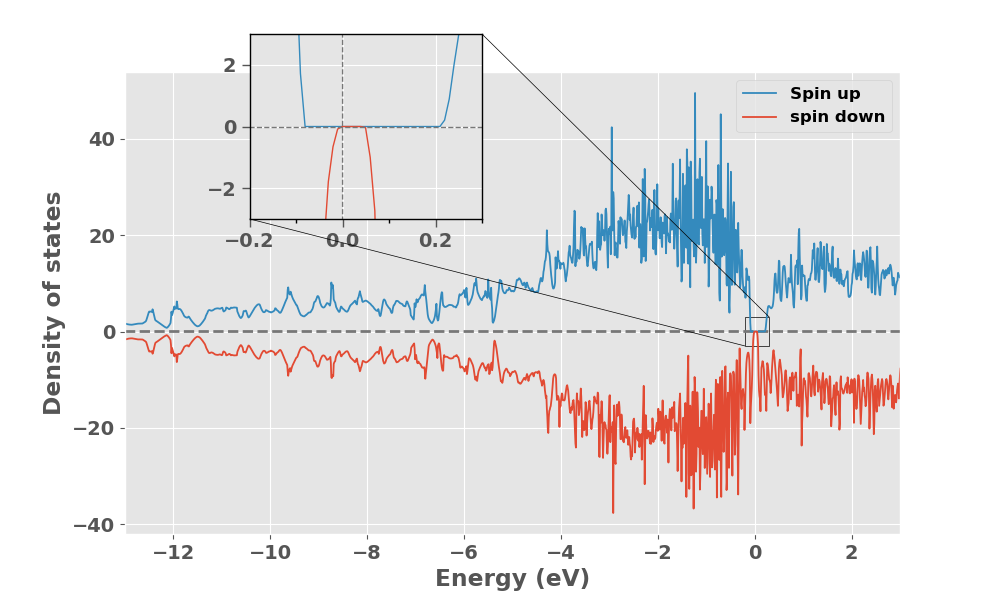
\includegraphics[width=\textwidth]{results/fesi2/B_TDOS.png}
	\caption{Density of states SQS B CFMN (fesi2) from PBE calculation}
\end{figure}

Above we have plotted the density of states of SQS B of this compound, here clearly showing a band gap in both spin channels. Similarly, also this SQS have a spin-polarized band gap, in spin up we see a band gap of around 0.3 eV, while the spin down states have a lesser band gap of 0.05 eV. This is a common trend of all SQSs excluding D of this composition. In table .. we list the band gap in both spin channels and the resulting total gap of all 5 SQSs. 

\begin{table}[H]
\centering
\begin{tabular}{@{}cccc@{}}
\toprule
Structure  & Spin-up & Spin-down & Total  \\ \midrule
\textbf{A} & 0.0814  & 0.0522    & 0.0281 \\
\textbf{B} & 0.2932  & 0.0523    & 0.0523 \\
\textbf{C} & 0.2355  & 0.0343    & 0.0343 \\
\textbf{D} & 0.3386  & 0         & 0      \\
\textbf{E} & 0.3078  & 0.0495    & 0.0495 \\ \bottomrule
\end{tabular}
\caption{Band gap (eV) with PBE in spin up and spin down channels of CFMN (fesi2) SQSs}
\end{table}

The density of states is a widely used and an insightful tool to learn about the character of a solid. For instance we can clearly see the magnetic character of the alloys and the magnitude of the band gap from the above plots.\textbf{What more can we say about the density of states? Find articles}. In the context of DFT and VASP however, the DOS include several factors that may contribute to inaccurate and sensitive results. As mentioned in section .., the type of numerical smearing is paramount for accurate DOS calculations. In this project we experienced large differences between calculations from gaussian and TBS smearing in relation to the band gap and DOS, this will be covered in more detail later. Moreover the DOS is very sensitive to computational factors such as the number of points in the DOS (NEDOS in VASP) and the number of k-points (to solve the DOS integral, see section ..). For example, the band gap in structure C could only be seen in the density of states when increasing the number of points in the DOS from 2401 to 20000 points. This is shown bellow in figure blabla, where we plot the density of states around the fermi energy, denoted by the strippled red and blue lines, relative to the density of states with 2401 points and 20000 points respectfully, all other parameters remained unchanged, it should however be noted that the second calculations applied the charge density calculated by the former for quicker convergence. 

\begin{figure}[H]
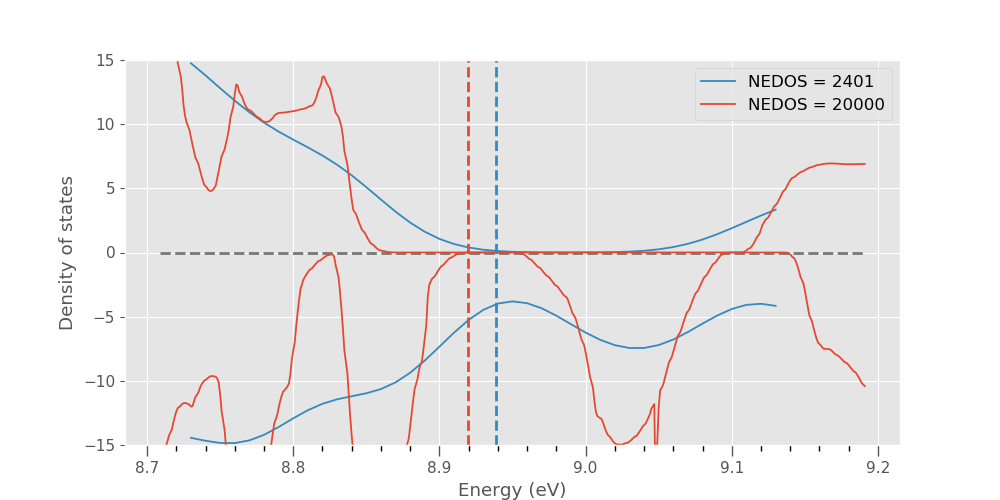
\includegraphics[width=\textwidth]{results/fesi2/C_DOS.png}
\end{figure} 

Despite of the higher accuracy of the greater number of points, we continue to perform calculations with 2401 points in most calculations, mostly down to the increased workload for analyzing and producing DOS related results with such a large number of points, and the use of vaspkits tools. 
 
A more secure method of evaluating the band gap is to consider the Kohn-Sham eigenvalues. The eigenvalues are provided for all energy bands for the given number of k-points used in the calculation, with listed energies and corresponding occupancy in both spin channels. The values listed in table (..) above was calculated from the eigenvalues. In addition to validate and provide an additional measure to the density of states, we can qualitatively differentiate SQS D. For certain k-points the occupancy does not transition from 1 to 0 directly between two bands, but rather contain one or more partially occupied bands in between (\textbf{Visualize? type fermi-dirc plot}), however only in the spin down channel. If we were to neglect these partially occupied states and only consider bands where the occupancy is above 0.99 or bellow 0.01, the band gap of structure D remain consistent in spin up, but we now observe a band gap of around 0.05 eV in the spin down channel resulting in a total band gap in the structure. Again, this would have been extremely insightful to investigate with the help of a band structure diagram.

\textbf{Something on the flaws of EIGENVALUES, bloch corrections yield un-physical eigenvalues in structures without band gap. Some times we find band gap from eigenvalues but not DOS or other script. What does the distance between up and down 1 occ and 0 occ mean?} 

\subsection{Meta-GGA and hybrid functional}

As expressed previously, in this work we involve 3 level of depths GGA (PBE), meta-GGA (SCAN) and hybrid functionals (HSE06) to determine the band gap of the SQSs. In table .. bellow we list the respective band gaps of these methods for all 5 SQSs of CFMN (fesi2). Note that all calculations is done with TBC smearing.

\begin{table}[H]
\centering
\begin{tabular}{@{}cccc@{}}
\toprule
Structure  & PBE    & SCAN   & HSE06  \\ \midrule
\textbf{A} & 0.0281 & 0.0000 & 0.0207 \\
\textbf{B} & 0.0523 & 0.0890 & 0.1808 \\
\textbf{C} & 0.0344 & 0.0690 & 0.0196 \\
\textbf{D} & 0.0000 & 0.0000 & 0.0000 \\
\textbf{E} & 0.0495 & 0.1048 & 0.0133 \\ \bottomrule
\end{tabular}
\caption{Band gap of CFMN (\ch{FeSi2}) SQSs with GGA (PBE), meta-GGA (SCAN) and hybrid-functionals (HSE06).}
\end{table}

\textbf{Need a comment on why we use the SCAN functional exactly, answer: Considered accurate, fast, and allows for testing on a level between gga and hybrid. Write this in the method section.}

The most obvious result of table .. is that aside from SQS A, all 3 methods agree on the presence of the band gap. This in itself is a very positive result for this project, as the primary motivation is based simply on locating semiconducting high-entropy silicides and thus the agreement of 3 different methods on the same structures is most welcome. On the other hand, it's clear that the actual size of the gap is under some debate. We note the largest observed band gaps is largely associated with the SCAN functional, compared to PBE calculations this result is very in line with what is expected by involving more complex factors in the calculations, as discussed in section .. In contrast, by the same argument we would not expect that par SQS B, the overall smallest band gaps is found with the well-proven hybrid functional HSE06, as shown in table .. The results associated with the HSE06 functional will be covered in more detail in the subsequent section, for now lets consider SCAN. 
 
\paragraph{SCAN \\}
For the most part, the results with SCAN meta-GGA prove similar to PBE, as was the case in the bulk material. The one exception is in SQS A. In this case the SCAN calculations result in a metallic character as opposed to the 0.03 eV band gap from PBE (0.08 eV up, 0.05 eV down). Upon investigating we discover that the eigenstates is riddled with both partial occupancy and so-called non-physical values. If we were two neglect these states, we find a band gap of 0.031 eV, very in line with the PBE result \textbf{Should I include this? I don't know why or what this means. And I don't really wanna spend a significant portion on one result with SCAN.} Other noteworthy concerns about the SCAN functional is apparent in the results of SQS C and D. \textbf{Explain from figure and state that C is identical, maybe include fiugre for this as well} \textbf{What more can I say about this? }

\textbf{Plot DOS C with PBE and SCAN side by side or like NEDOS around Ef to show the difference. Also make one for E to show how SCAN decrease the spin up gap and increase the spin down gap.}       
\textbf{Mention that the transistion is different for PBE and SCAN of the same structure in every SQS.}

Don't need more words to explain the results of SCAN for B and E, let the figures do the talking here. Need a conlusion on SCAN, but I can savour this to the conclusion bellow.

\paragraph{HSE06 \\}
\textbf{Wait for jobs to finish: lesssmear and ismear0}
As stated above, the measured band gaps with the HSE06 functional was less than that of PBE and SCAN for most of the tested SQSs. Hybrid functionals as described in section .. is computationally demanding, but comes with superior accuracy for band gap measurements, and the HSE06 functional in particular is on the top of the list. For this reason, one would in general expect larger band gaps compared to GGA or meta-GGA calculations, as highlighted in .. \textbf{cite?} The one exception we observed to this trend is in SQS B, here the band gap increase from 0.05 eV to 0.09 eV and 0.18 eV from PBE to SCAN to HSE06. One possible reason behind the abnormally large gap can originate from the small number of k-points we had to employ in order for the calculations to converge. Recalling that the gap transition in in the PBE calculation was (0.250,0.000,0.250)-(0.000,0.000,0.000), compared to the hybrid functional we now see that the transition is between k-points (0.500,0.000,0.000) and (0.000,0.000,0.000). Moreover, the point (0.250, 0.000, 0.250) in k-space is not included in the hybrid functional due to the narrow mesh (this we read from the IBZKIT file in VASP). Thus it's a possibility that the large gap is caused by the fact that the minimal gap is not encapsulated by the k-points in the HSE06 calculation. However we also see this trend in the other SQSs, but despite of the different transistion in k-space, these structures find lesser band gaps with the HSE06 functional compared to PBE. Additionally, we find similar results in the bulk $\beta-$\ch{FeSi2} structure. In this calculation we applied the same number of k-points for HSE06 as for PBE and SCAN. Nevertheless we find a much larger band gap of around 1.5 eV with HSE06, as opposed to 0.65 eV with both PBE and SCAN, and as mentioned before the two latter is in much better agreement with experimental results and ab intio work on the band gap of $\beta-$\ch{FeSi2} \textbf{cite materials project, other articles}. Additionally also in this case, the transition vary between functionals. PBE: (0.000,0.000,0.000)-(0.000,0.000,0.250), and HSE06: (0.000,0.000,0.000)-(0.000,0.000,0.500). \textbf{Include band-diagram for bulk fesi2?} 

\textbf{Mention HSE06 results, then briefly mention smearing}

In the HSE06 calculations we noticed a pattern between all five supercells. We will use SQS A to explain this concept, and then briefly list the relevant results of the remaining SQSs.In A we calculate a band gap close to 0.021 eV, from the eigenvalues we know that the gap is 0.7 eV in the spin up, and 0.02 eV in spin down \textbf{See DOSCAR maybe?}. As discussed in section .., in order for the HSE06 calculations to converge we had to first perform a self-consistent run with Gaussian smearing, then reapply the calculated charge density to perform subsequent calculations with TBC smearing. Between the two we can report large differences in the calculated band gap for almost all SQSs. From the former (Gaussian), the band gap of SQS A is 0.15 eV, (0.78 up and 0.15 down). However the eigenvalues contain defect states and the band gap is not completely observable from the density of states. \textbf{Figure?} By reducing the gaussian smearing width from 0.05 eV to 0.005 eV we find a new gap of 0.1 eV (0.21 up and 0.1 down), now the eigenstates are clean of defects, but still not obvious from the density of states \textbf{figure}. The point we are trying to make here is that the band gap associated with the HSE06 calculation is sensitive to both the smearing type, and width in the case of gaussian smearing. In addition to the density of states and eigenvalues, we use the script bandgap.py of the pymatgen package to check the band-gap of a structure, refer to section .. for a description of this script. The script only return a band gap for the HSE06 calculation with TBC smearing, similar to the density of states. 

\textbf{Create figure/subfigure of the DOS of hybrid/smear/smear5 calculations to illustrate the above point}

In contrast to this case, the smearing type have minimal affect on the results of SQS B. With the PBE functional (TBC) this supercell show a band gap of 0.3 eV in spin up, and 0.05 eV in spin down, see table 8.3 and figure 8.3. From HSE06 calculations we find a band gap of 0.29 eV and 0.18 eV in spin up and down respectfully, and 0.18 eV in total. Noteworthy of this result is that applying gaussian smearing with both 0.05 and 0.005 eV results in 0.28, 0.18 and 0.18 eV as the spin up, down and total band gap as for TBC smearing, but similar to sqs A, the larger smearing width comes with a few defect states in the spin down channel and additionally can not be seen in the density of states. As a last point regarding the band gap of this SQS in terms of the smearing method, the same exact trend is found between gaussian and TBC smearing with the PBE functional. \textbf{Wait for toten/lesssmear B to finish}  The hse06 lesssmear calculation finds a bandgap from eigenvalues (no defects) and the bandgap.py script, but the density of states is slightly off centered in regards to Ef, and with the larger smearing width, the DOS is very small around E_f but not zero as it is for TBC. I don't think this is a property of the method, but the consequence of the accuracy in the DOS in TBC vs gaussian. The large width contains defects in down, but all 3 show very similar values in up and down.

Structure C is similar to B with PBE, where the smearing method produce similar band gaps, but the gaussian contain defect states. HSE06 agree with PBE, and find that the spin up channel have a band gap of 0.17 eV and 0.032 eV in spin down. With gaussian smearing, we find HSE06 to yield a gap around 0.1 eV in both channels and 0.065 eV in total (with defect states).

In structure D, The results of HSE06 for this supercell is similar to structure C, in agreement with PBE and disagreement with SCAN. The band gap from HSE06 is calculated to about 0.37 eV in up and 0 in down from TBC smearing. \textbf{Wait for ismear0 HSE06 to finish}. 

Structure E. The PBE functional find a large gap in up and near 0 in down with TBC smearing. And the gaussian smearing find a similar gap in spin up, and the small gap in spin down is consistent, but caused by defects. The HSE06 calculations of this structure resemble that of structure A. With TBC, the band gap is very large in spin up, about 0.55 eV, but close to 0 in down. The gaussian smearing finds similarly a large gap in up (0.66 eV) and a larger spin down gap around 0.15 eV, with defect states and 0.16 eV without. This gap is not apparent in the density of states, but we have found merit that the gap could become viable, by reducing the smearing width, as in structure A.  

\textbf{Compare HSE06 to PBE (and SCAN?) similar charactheristics ie spin up down relationship more important to values. How does smearing impact pbe vs hse results. Important to go through this section again and rewrite contains defects to contains defects in spin channel ..}

\textbf{Include here a figure or number on the computation time between PBE, SCAN and HSE06.}
\textbf{Make a figure to illustrate the difference between smearing type and one for functionals.}  
\textbf{Do I need to list all values of the gap: spin down, up for all functionals, smearings, SQSs etc? If so where/how?}
\textbf{something on the number of defect states, seem like here we find few defect states and still find a band gap, but in others the number increase and so the gap vanishes.} 
\textbf{Conclusion of this section on functionals and the band gap: Question: Which method/functional/smearing/etc should we trust?}
We see that the results vary greatly between both PBE, SCAN and HSE06, as well as withing the functionals. We observe several uncertainties revolving the SCAN and HSE06 jobs, such as disagreement with PBE and spin polarization in SCAN, see SQS A, C and D with SCAN. And the problamatic smearing dependence in HSE06, that we do not experience in PBE. Combining this with the popularity and wide-spread application and reliability of the PBE functional. See for example materials project, that exclusivly list PBE band gaps, and other relevant studies. We put the most faith in the PBE results. An additional point is that GGA is known to underestimate band gaps, due to the concepts described in section .., therefore we can conclude that if we find a gap with PBE, the real material would most probably also have a band gap, and a larger one at that. Similarly, the HSE06 is the most well-known functional for accurate band gaps, but due to the large computational requirement and the complex structures of this project, we had to perform these both creatively and scarcely, thus we could not obtain rigid results through a large scope of tests and calculations with the functional. Also, in the cases where we could perform comperative HSE06 (To PBE), this functional produced some surprising results that seem to deviate more from experimental baselines than SCAN and PBE. Actually, we found that PBE produced best in this case. That is also a factor to consider in this project, namely that the lack of an experimental baseline to compare and meassure our results after. Lastly, the fact that all 3 functionals agree on the presence and charachter of the structures is a good result in itself. A qualitative study on the exact band gap would demand a much greater focus and testing, as there are many factors affecting the value that we have neglected. In addition, the concept of SQSs involve an element of randomness, therefore even with exact numerical meassurements, the value would still be prone to inaccuracies. For instance, by increasing the SQS size, ie number of atoms in the supercell, we found completly different band gaps, but still, the presence and characther of the compound is of the upmost importance in this study. \textbf{Maybe include results from varying SQS size here? To draw any meaningfull conclusions on the size of the band gap would requiere us to both increase the number of SQS's of the composistion due to the obseved variation in the band gap between the 5 tested supercells. Additionly, we would have to do this as well for different supercell sizes to obtain some sort of convergence of the band gap. Obviously this appears as a very demanding on long task to complete. And the focus of this project was to provide a broad search of such materials, rather than the in-depth qualitative direction desrcribed above for one particular system. Additional point in conclusion on which functional is most reliable, this must be a comprimise between experimental comparisons (bulk), computational efforts, and most sensible. An unrelevant result I may want to include is that in terms of smearing, the calculation of forces was way of with TBC, as vaspwiki stated regarding relaxation of metals, maybe this is an indication of that the practical and theoretical are in agreement, thus TBC should be the prefferred result of the bandgap and DOS. Conclusion on the band gap, ie we find overwhelming proof that the hypothetical alloy is semiconducting, or due to the large spin polarization we may label it as a half-metal or a spin-gapless condutor which would apply the material for many interesting and relevant applications, such as spintronics or spin dependent semiconductors etc etc. We also find that the PBE and HSE06 agree completly on the charachter of the material, but differ in values, while the results of SCAN was more conflicting. Examples are A, PBE and HSE06 both find large gaps in up, HSE most, and small in down.
From the general concencious these are also the two most popular functionals for studying the band gap of the material due to one, the cheap nature of GGA, and the accuracy of HSE06, meanwhile SCAN is somewhere in the middel both in terms of accuracy and cost. All though we find that the SCAN functional is actually less accurate than PBE. See for example bulk fesi2 and SQS A, C, and D. One possible result is that hse06 better predict the half-metal behaviour, ie finds large gaps in up, but want the down channel more to be zero I guess.}

\subsection{Probability distribution functions and charge density}

If we now consider the probability distribution functions (PDFs), shown in figure \textbf{insert ref!}. From these figures there is a lot of useful information to investigate. With the aid of the ICSD (insert citation), we can locate the expected PDFs based on recent research and experiments from a host of different compounds. As our compound contain a total of 15 different bonds, comparing each one of these for all 5 supercells to the ICSD values would be an exhaustive process. For our purpose we are satisfied by comparing the 4 different metal-Si bonds and note ourselves of key distinctions. We find that the preferred bond-length of TM-Si is observed at two values, the most dominant being the shorter of the 2. For Fe-Si these are between 2.25-2.75 and 4-5, Mn-Si 2.25-2.75 and 3.5-5. Ni-Si lie between 2.25-2.5 and 3.85-5 and Cr-Si between 2.35-2.65 and 4-5. 

\begin{figure}[H]
	\centering
	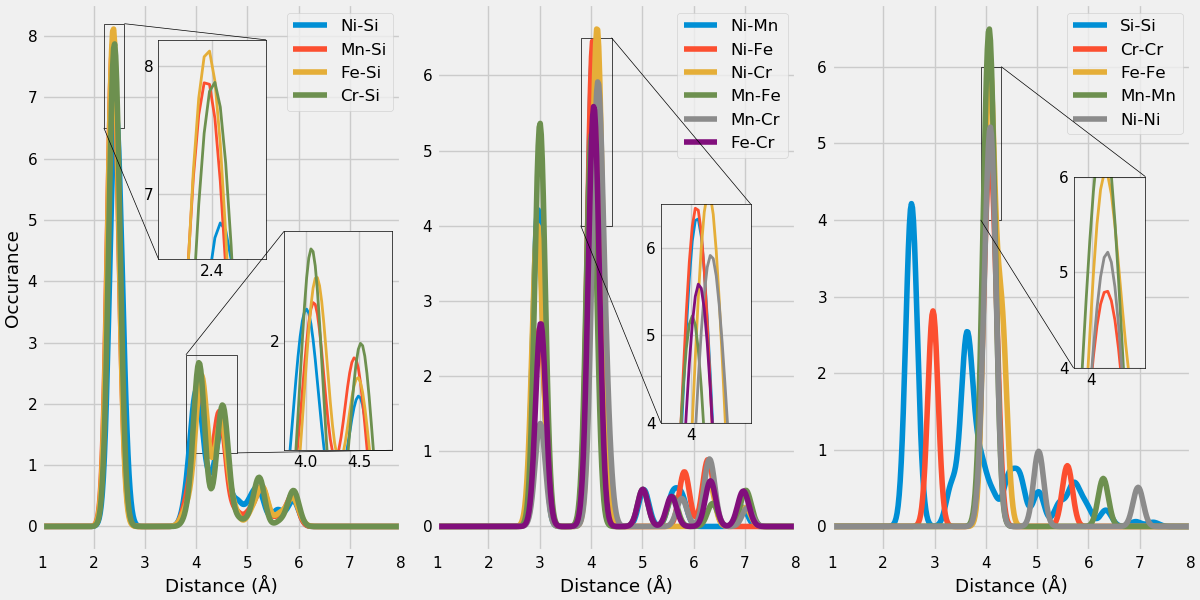
\includegraphics[width=\textwidth]{results/fesi2/D_PDF2.png}
\end{figure}

\begin{figure}[H]
	\centering
	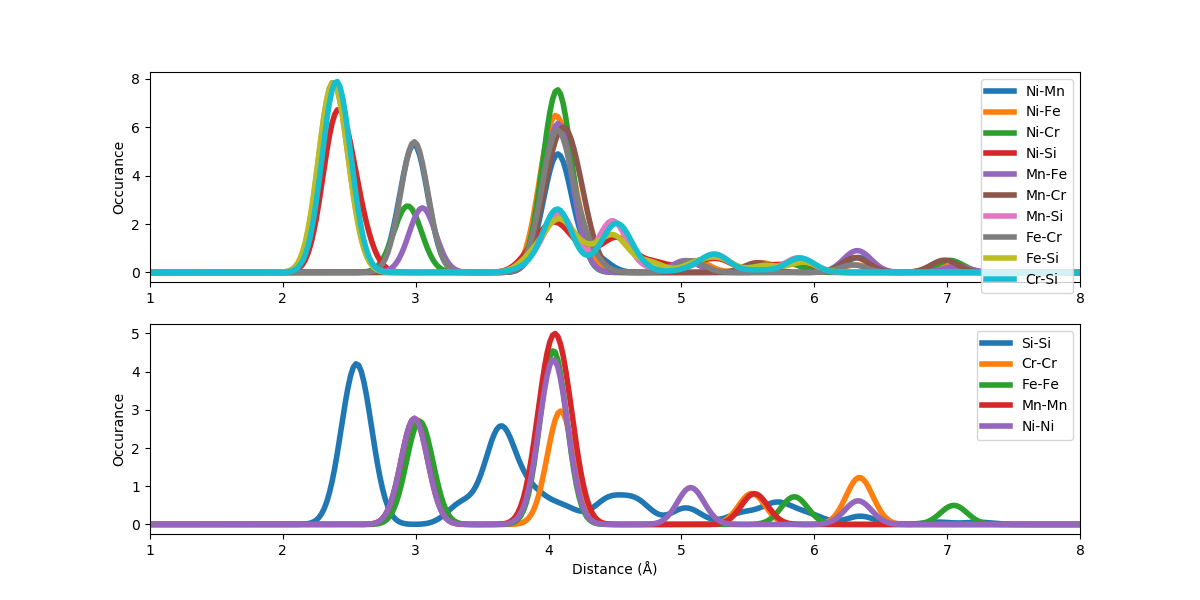
\includegraphics[width=\textwidth]{results/fesi2/B_PDF.png}
\end{figure}

\begin{figure}[H]
	\begin{subfigure}{.5\textwidth}
		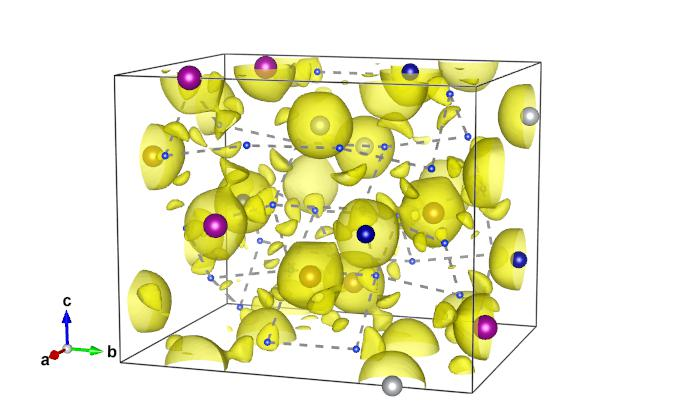
\includegraphics[width=\textwidth]{results/fesi2/B_CHGCAR.jpg}
		\caption{Structure B}
	\end{subfigure}
	\hfill
	\begin{subfigure}{.5\textwidth}
		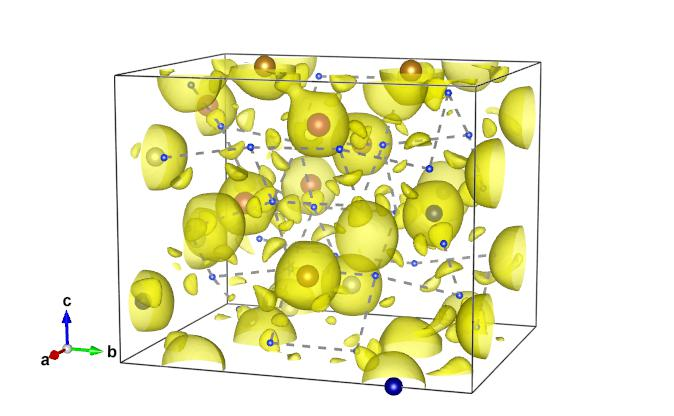
\includegraphics[width=\textwidth]{results/fesi2/D_CHGCAR.jpg}
		\caption{Structure D}
	\end{subfigure}
\end{figure}

At the surface, figure .. show that are supercells are in good agreement with the listed values for Tm-Si bonds, with the most occurring bond length falling at around 2.4 Å for all TMs, and some bonds at around 4.1 Å. The relative height of the peaks follow a similar trend, Fe-Si, Mn-Si, and Cr-Si all lie close to 8 for the first peak at 2.4 Å, and Ni-Si slightly bellow around 7. \textbf{More on the PDFs?}

Lastly we include the charge density of blabla, \textbf{something on these.}

\section{Permutations}

Up until this point we have investigated the structure CFMN (\ch{FeSi2}). Morre specificly we have looked at the center of a quasiternary pahse diargram. In this section, we aim to exapand our search of this diargram by studying SQSs slightly away from eqvimolar distribution of 3d elements. In table (bellow) we list the mean total energy and magnetic moment per atom with corresponding standard deviation, and enthalpy of formation of 4 different permutations of the quasiternary phase diagram. Ideally we would like to only alter one element at a time, but the TDEP method insist in also reducing Nickel to stay consistent with the 48 atom supercells. The 4 permuations are listed bellow

\begin{table}[h!]
\centering
\begin{tabular}{@{}cccccc@{}}
\toprule
       & \multicolumn{2}{c}{Toten (eV)} & Enthalpy of formation & \multicolumn{2}{c}{Mag} \\ \midrule
\ch{Cr3Fe3Mn7Ni3Si32} & 6.6947      & 0.0040 & -11.9586      & 0.1375     & 0.0186     \\
\ch{Cr5Fe5Mn3Ni3Si32} & 6.6705      & 0.0030 & -11.1991      & 0.1127     & 0.0223     \\
\ch{Cr5Fe3Mn5Ni3Si32} & 6.6852      & 0.0041 & -10.5200      & 0.1375     & 0.0456     \\
\ch{Cr3Fe5Mn5Ni3Si32} & 6.6801      & 0.0036 & -12.6426      & 0.0937     & 0.0209     \\ \bottomrule
\end{tabular}
\caption{Mean and stadard deviation of the total energy and magnetic moment per atom, plus enthalpy of formation of the listed mean energies (\ch{FeSi2}).}
\end{table}

Interestingly we find that we can increase the stability of the compound by adjusting the distribution of 3d elements. The most stable permutation is found when we increase the amount of manganese relative to the other TMs. In said permutation we find very similar properties as the equal distribution in terms of the band gap. From PBE calculations, we find that the band gap ranges from 0.13-0.47eV in spin up, depending on the supercell and all except for structure D have zero gaps in down, here we find a total band gap of 0.0063 eV. In contrast to equally distributed CFMN (fesi2), the SCAN functional does not find a band gap in any of the five supercells, except for small gaps less than 0.06 eV in spin up for structures D and E. Extending to the HSE06 functional, we find that structre D contain a large band gap of 0.17 eV, 0.57 eV and 0.26 eV in spin up and down respectfully. Both the gaussian and TBC smearing method are in excellent agreement of the gap. Howver, the result of the hybrid functional are surrounded by the same factors of uncertainty as described for CFMN (fesi2), in that also in this case we find that the transistion of the indirect band gap is sensetive to the applied functional and escpecially the limited number of k-points used to perfrom HSE06 calculations.

If we now move in the opposite direction and reduce the number of manganese atoms we observe the opposite, namely the least stable permutation in terms of the total energy. One of the 5 SQSs (D) is a semiconductor, this supercell show from PBE calculations a band gap of 0.067 eV (up) and 0.041 eV (down) and 0.037 eV in total. The SCAN functional in contrast predict a half-metal with a band gap of 0.17 eV in spin down. The conflicting band gap contunue with the HSE06 functional, resulting in 0.77 eV in spin up and 0.22 eV in down and total. Thus PBE and HSE06 result in a semiconductor with HSE06 pointing to a large spin polarization and PBE finding symetric spin values. And on the other side, meta-GGA calculations predict a half-metal with semiconduction in the spin-down channel, opposiste of the polarization from HSE06. As follows drawing a conclusion on the band gap is challanging, but as discussed previosly we emphazie the results of GGA and hybrid functionals for the univeral application and reputation they hold in self-consistent method studies of electronic structure. 

The two most stable SQSs C and E, both exhibit large band gaps soeley in the spin up channel. These gaps contain a few partially occupied bands that result in the gap vanishing in the density of states. This is an interesting result, as opposed to structures where many bands are partially filled, the structure is obviosuly a metal as apperant from both the calculated band gap and density of states. But in cases where there are only very few states with partial occupation we see a band gap from the eigenvalues and also the density of states show indication of a band gap with the DOS becomming very low near the fermi energy, but not exactly zero as in the structures with no partial occupants.\textbf{Include DOS figure??} The spin up band gap in C and E discussed above is calculated from the eigenvalues as 0.21 and 0.36 eV respectfully. In both cases the gap vanishes with SCAN, and HSE06 calculates unfortunatly proved difficult to converge for these structures, thus we were unable to obtain results with the hybrid functional. A positve conclusion of this permutation, is that if we include the possible half-metal gaps in C and E, we can report that the most stable arrangements are half-metals, then semiconducting and the least stable SQS is metalic. In conclusion we can then state that semiconducting and escpecially half-metalalic are the preffered state over metallic in this permutation.     

\ch{Cr5Fe3Mn5Ni3Si32} is on par with \ch{Cr5Fe5Mn7Ni3} in terms of both stability and magnetism. We note that the high magnetic moment is mostly attributed to the least stable SQSs, and the more stable arrangements have magnetic moment 5/48, as opposed to the first permutation in which we found high magnetism also in the stable SQSs. From PBE GGA calculations we obtain spin-polarized half-metals in structures A, B, C, and E with the spin up gap ranging between 0.21(A)-0.47(C) eV. Wheras structure D is a semiconductor with a 0.012 ev band gap (slightly larger in up than down). Additionaly this is also the most stable SQS second only to A. In most cases, the use of SCAN results in very small spin up gaps, the rest 0. From the hybrid functional we find very conflicting results of strcture D. With TBC smearing, HSE06 predict a metalic gap , but  we see signs in the density of states that may indicate a half-metal in spin down \textbf{Figure?}. Using instead the gaussian smearing method results in a gap of 0.063 eV and 0.27 eV in spin down with some partial occupancy in both channels, but much rarer and less impactfull in the spin down states (Similar DOS as TBC).        

Lastly, the final permutation we did of CFMN (fesi2) was to reduce the amount of Cr. The most dominant display of this is the magnetism, out of the 4 permutations and the baseline system, this was the least magnetic system, according to our calculations with a fixed magnetic configuration. This is not a surprising result recalling that in CFMN fesi2, the magnetic momemt was primarly attributed to Cr atoms in the lattice. We find 2 semiconductors (D and E) and 2 half-metals (A and C). Similar to the other systems discussed in this section, the half-metals display a sizable band gap in the spin up direction, 0.39 eV and 0.12 eV respectfully. SCAN calculations result in stucture A being a semiconductor with a band gap of 0.015 eV, and B a metal. Of the two semiconductors, both PBE and SCAN agree of a band gap, PBE predict a band gap of 0.1 eV (0.25 up and 0.1 down) in D, and 0.014 eV (0.21 up and 0.08 down) with SCAN. In contrast to both, HSE06 calculations produce a semi-metal with a spin up gap of 0.53 eV. In E we find a band gap of 0.35 and 0.10 eV in the two spin directions, yielding a total gap of 0.084 eV. The SCAN calculations find several nonphysical eigenstates and thus no band gap. From HSE06, we find as before greatly exatereded band gaps of 0.74 eV in spin up, and 0.25 eV in total. An additiontal positive regarding this permutation is that the two semiconducting SQSs are the most stable of the set, with D having the highest total energy, followed by E. The least stable supercell is A, it's important to note however that the total energy very similar across all SQSs as seen from the standard deviation in table .. 

\begin{table}[h!]
\centering
\begin{tabular}{@{}ccccc@{}}
\toprule
                                                     &   & Spin up (eV) & Spin down (eV) & Total (eV) \\ \midrule
\multicolumn{1}{c|}{\multirow{5}{*}{\textbf{\ch{Cr3Fe3Mn7Ni3Si32}}}}   & A & 0.3390                & 0                       & 0                   \\
\multicolumn{1}{c|}{}                                & B & 0.4745                & 0                       & 0                   \\
\multicolumn{1}{c|}{}                                & C & 0.1342                & 0                       & 0                   \\
\multicolumn{1}{c|}{}                                & D & 0.1950                & 0.0063                  & 0.0063              \\
\multicolumn{1}{c|}{}                                & E & 0.4211                & 0                       & 0                   \\ \midrule
\multicolumn{1}{c|}{\multirow{3}{*}{\textbf{\ch{Cr5Fe5Mn3Ni3Si32}}}} & C & 0.2103                & 0                       & 0                   \\
\multicolumn{1}{c|}{}                                & D & 0.0674                & 0.0413                  & 0.0372              \\
\multicolumn{1}{c|}{}                                & E & 0.3619                & 0                       & 0                   \\ \midrule
\multicolumn{1}{c|}{\multirow{5}{*}{\textbf{\ch{Cr5Fe3Mn5Ni3Si32}}}} & A & 0.2082                & 0                       & 0                   \\
\multicolumn{1}{c|}{}                                & B & 0.4053                & 0                       & 0                   \\
\multicolumn{1}{c|}{}                                & C & 0.4659                & 0                       & 0                   \\
\multicolumn{1}{c|}{}                                & D & 0.0843                & 0.0121                  & 0.0121              \\
\multicolumn{1}{c|}{}                                & E & 0.3008                & 0                       & 0                   \\ \midrule
\multicolumn{1}{c|}{\multirow{4}{*}{\textbf{\ch{Cr3Fe5Mn5Ni3Si32}}}} & A & 0.3922                & 0                       & 0                   \\
\multicolumn{1}{c|}{}                                & C & 0.1285                & 0                       & 0                   \\
\multicolumn{1}{c|}{}                                & D & 0.2595                & 0.1004                  & 1.004               \\
\multicolumn{1}{c|}{}                                & E & 0.3591                & 0.1003                  & 0.0848              \\ \bottomrule
\end{tabular}
\caption{Total and spin polarized band gap of 4 permutations of CFMN (fesi2) with PBE GGA calculation. The structures that are excluded from this list either failed in calculations, or does not show any band gap.}
\end{table}

In this section we have seen that it's defintivly a merit for exploring the quasiternary phase diagram. We find the overall most stable composistion by increasing the number of manganese atoms in the composistion. Judging from the most stable supercells of the permutations, we can say that the high magnetic moment is attributed to chromium and manganese atoms as in the CFMN (fesi2) system. The same can be saif for the \ch{Cr5Fe3Mn5Ni3Si32} alloy where we increase the proportions of the magnetic elements Cr and Mn relative to Fe and Ni. From these patterns observed in the permutations and the equal distribution of CFMN (fesi2), we can conclude that the magnetic properties of this compound is reliant on chromium and manganese. This is also seen from the magnetism in the permutations where we reduce these elements, ie low magnetic moment. \textbf{Something on why one is more stable than the other, and why they all are more stable than equal dist.}

With reference to the band gap, we see from table .. that half-metalic is the most preferred state in most permutaions. This is in line with the eqvimolar distribution, as also here we observed severe spin polarization, mainly spin up, in addition to the semiconducting character. As was the case in CFMN (fesi2), we can not report any concise relation between the stability of the supercells and band gap, except for that the semiconducting SQSs is rarely the most stable of the set, but always above the mean total energy, the exception for this obviosuly being the chromium reduced alloy in which the two highest energy SQSs both were semiconductors. An interesting observation of the band gap is the relation to the magnetic moment. From table .. we see that the permutations differ in magnetic moment, but internly as highligted by the standard deviation we also note a variation in the magntic moment. And facinatingly, all reported semiconductors have the identical magnetic moment equal to 5.0000/48. The only exception is the eqvimolar system, were all structures had identical mag equal to 4.0000/48. Howver, this observation does not point to any domintating direction as this value is not the minimum or maxium magnetization, so we can not report a relation between high/low magnetization and the band gap.         

As a conclusion to this segment we do not find one best direction to expore of the quasiternary phasediagram, as good and promising results was unveiled to some degree in all directions. This definitivly motivates the further exploration of the diagram, with the prospect of both improving the properties of the eqvimolar system and the ability to tune the properties by going in certain directions. In respect to the band gap, the most promising direction seems to be along manganese, as we see the most frequently large band gaps (in spin up) by increasing manganese, and the least frequent by reduction of manganese. For purely semiconducting compounds, reduction of chromium appears as a viable option seen from the $50\%$ ratio of semiconducting to half-metalic ratio. An intersting proposistion for future work would thus be to reduce chromium and increase manganese simontainusly. 

\textbf{Conclusion example: In this project we have found many structures that show signs of semiconducting properties, but only CFMN fesi2 produced clear indication thorugh all 3 levels of meassures, ie eigenvalues, bandgap.py and dos, 3 levels of depth; PBE, SCAN, HSE06, and 5 levels of width, ie the 5 SQSs}

\textbf{Skriv i introducksjonen av resultater intensjonen vår med å nevne ting som stabilitet og magnetisme, og hvor overfladisk den analysen her. En ordentlig analyse av dette ville involvert mange flere jobber med ulike magnetiske konfigurasjoner og innstillinger. En stabilitetsavhandling ville invlovert grundigere relaksering og analyse av gitterparametere og celle, finite temperatur beregninger osv. Hovedvekten i denne oppgaven er på båndgapet}